

\tikzset{every picture/.style={line width=0.75pt}} %set default line width to 0.75pt        

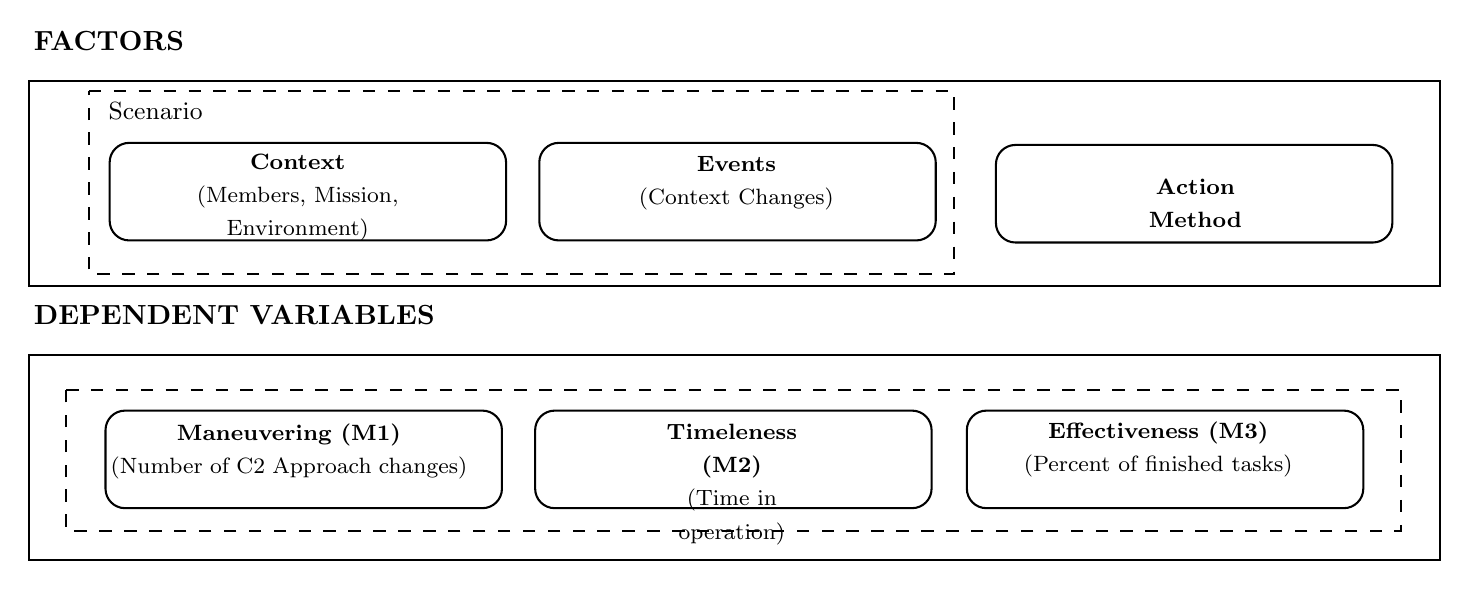
\begin{tikzpicture}[x=0.75pt,y=0.75pt,yscale=-1,xscale=1]
%uncomment if require: \path (0,511); %set diagram left start at 0, and has height of 511

%Shape: Rectangle [id:dp2552012932916572] 
\draw  [color={rgb, 255:red, 0; green, 0; blue, 0 }  ,draw opacity=1 ] (11,101) -- (691,101) -- (691,200) -- (11,200) -- cycle ;
%Rounded Rect [id:dp9161828495455207] 
\draw   (50,140.4) .. controls (50,135.21) and (54.21,131) .. (59.4,131) -- (231.6,131) .. controls (236.79,131) and (241,135.21) .. (241,140.4) -- (241,168.6) .. controls (241,173.79) and (236.79,178) .. (231.6,178) -- (59.4,178) .. controls (54.21,178) and (50,173.79) .. (50,168.6) -- cycle ;
%Rounded Rect [id:dp47914804412585] 
\draw   (257,140.4) .. controls (257,135.21) and (261.21,131) .. (266.4,131) -- (438.6,131) .. controls (443.79,131) and (448,135.21) .. (448,140.4) -- (448,168.6) .. controls (448,173.79) and (443.79,178) .. (438.6,178) -- (266.4,178) .. controls (261.21,178) and (257,173.79) .. (257,168.6) -- cycle ;
%Rounded Rect [id:dp36207445324802223] 
\draw   (477,141.4) .. controls (477,136.21) and (481.21,132) .. (486.4,132) -- (658.6,132) .. controls (663.79,132) and (668,136.21) .. (668,141.4) -- (668,169.6) .. controls (668,174.79) and (663.79,179) .. (658.6,179) -- (486.4,179) .. controls (481.21,179) and (477,174.79) .. (477,169.6) -- cycle ;
%Shape: Rectangle [id:dp7958558916033278] 
\draw  [dash pattern={on 4.5pt off 4.5pt}] (40,106) -- (457,106) -- (457,194) -- (40,194) -- cycle ;
%Shape: Rectangle [id:dp34078076660428835] 
\draw  [color={rgb, 255:red, 0; green, 0; blue, 0 }  ,draw opacity=1 ] (11,233) -- (691,233) -- (691,332) -- (11,332) -- cycle ;
%Rounded Rect [id:dp614914351003329] 
\draw   (48,269.4) .. controls (48,264.21) and (52.21,260) .. (57.4,260) -- (229.6,260) .. controls (234.79,260) and (239,264.21) .. (239,269.4) -- (239,297.6) .. controls (239,302.79) and (234.79,307) .. (229.6,307) -- (57.4,307) .. controls (52.21,307) and (48,302.79) .. (48,297.6) -- cycle ;
%Rounded Rect [id:dp9126417804308116] 
\draw   (255,269.4) .. controls (255,264.21) and (259.21,260) .. (264.4,260) -- (436.6,260) .. controls (441.79,260) and (446,264.21) .. (446,269.4) -- (446,297.6) .. controls (446,302.79) and (441.79,307) .. (436.6,307) -- (264.4,307) .. controls (259.21,307) and (255,302.79) .. (255,297.6) -- cycle ;
%Shape: Rectangle [id:dp68280710046261] 
\draw  [dash pattern={on 4.5pt off 4.5pt}] (29,250) -- (672,250) -- (672,318) -- (29,318) -- cycle ;
%Rounded Rect [id:dp2824039190738554] 
\draw   (463,269.4) .. controls (463,264.21) and (467.21,260) .. (472.4,260) -- (644.6,260) .. controls (649.79,260) and (654,264.21) .. (654,269.4) -- (654,297.6) .. controls (654,302.79) and (649.79,307) .. (644.6,307) -- (472.4,307) .. controls (467.21,307) and (463,302.79) .. (463,297.6) -- cycle ;

% Text Node
\draw (12,76) node [anchor=north west][inner sep=0.75pt]   [align=left] {\textbf{FACTORS}};
% Text Node
\draw (56,135) node [anchor=north west][inner sep=0.75pt]   [align=left] {\begin{minipage}[lt]{124.70588000000001pt}\setlength\topsep{0pt}
\begin{center}
\textbf{{\footnotesize Context}}\\{\footnotesize (Members, Mission, Environment)}
\end{center}

\end{minipage}};
% Text Node
\draw (303,136) node [anchor=north west][inner sep=0.75pt]   [align=left] {\begin{minipage}[lt]{71.20892pt}\setlength\topsep{0pt}
\begin{center}
{\footnotesize \textbf{Events}}\\{\footnotesize (Context Changes)}
\end{center}

\end{minipage}};
% Text Node
\draw (532,147) node [anchor=north west][inner sep=0.75pt]   [align=left] {\begin{minipage}[lt]{59.38310800000001pt}\setlength\topsep{0pt}
\begin{center}
{\footnotesize \textbf{Action Method}}
\end{center}

\end{minipage}};
% Text Node
\draw (48,110) node [anchor=north west][inner sep=0.75pt]   [align=left] {{\small Scenario}};
% Text Node
\draw (12,208) node [anchor=north west][inner sep=0.75pt]   [align=left] {\textbf{DEPENDENT VARIABLES}};
% Text Node
\draw (49,265) node [anchor=north west][inner sep=0.75pt]   [align=left] {\begin{minipage}[lt]{128.81784pt}\setlength\topsep{0pt}
\begin{center}
{\footnotesize \textbf{Maneuvering (M1)}}\\{\footnotesize (Number of C2 Approach changes)}
\end{center}

\end{minipage}};
% Text Node
\draw (301,265) node [anchor=north west][inner sep=0.75pt]   [align=left] {\begin{minipage}[lt]{70.90088000000002pt}\setlength\topsep{0pt}
\begin{center}
{\footnotesize \textbf{Timeleness (M2)}}\\{\footnotesize (Time in operation)}
\end{center}

\end{minipage}};
% Text Node
\draw (489,264) node [anchor=north west][inner sep=0.75pt]   [align=left] {\begin{minipage}[lt]{97.05912000000001pt}\setlength\topsep{0pt}
\begin{center}
{\footnotesize \textbf{Effectiveness (M3)}}\\{\footnotesize (Percent of finished tasks)}
\end{center}

\end{minipage}};


\end{tikzpicture}